\documentclass[conference]{IEEEtran}

\usepackage{booktabs}
\usepackage{cite}
\usepackage[bottom]{footmisc}
\usepackage[utf8]{inputenc}
\usepackage{graphicx}
\usepackage{listings}
\usepackage{multicol}
\usepackage{newtxtext}
\usepackage{newtxmath}
\usepackage{url}
\RequirePackage[l2tabu, orthodox]{nag}

% Allow PDF 1.7 documents to be included with \includegraphics
\pdfminorversion=7

% listing
\lstset{%
  language={C},
  basicstyle={\small\ttfamily},%
  identifierstyle={\small\ttfamily},%
  commentstyle={\small\itshape},%
  keywordstyle={\small\bfseries},%
  ndkeywordstyle={\small\ttfamily},%
  stringstyle={\small\ttfamily},%
  frame={tb},%
  breaklines=true,%
  columns=[l]{fullflexible},%
  numbers=left,%
  numberstyle={\scriptsize},%
  stepnumber=1,%
  numbersep=1em,%
  lineskip=-0.5ex,%
  mathescape,%
  xleftmargin=2em,%
  framexleftmargin=1.5em,%
}

\begin{document}

\title{kEDM: A Performance-portable Implementation of Empirical Dynamical Modeling}

\author{%
    \IEEEauthorblockN{%
        Keichi Takahashi,\\ Wassapon Watanakeesuntorn,\\Kohei Ichikawa
    } \\
    \IEEEauthorblockA{%
        Nara Institute of Science and Technology\\
        Nara, Japan\\
        \{keichi, wassapon.watanakeesuntorn.wq0,\\ ichikawa\}@is.naist.jp
    }
    \and
    \IEEEauthorblockN{%
        George Sugihara
    } \\
    \IEEEauthorblockA{%
        University of California San Diego\\
        California, USA\\
        gsugihara@ucsd.edu
    }
    \and
    \IEEEauthorblockN{%
        Gerald M. Pao
    } \\
    \IEEEauthorblockA{%
        Salk Institute for Biological Studies\\
        California, USA\\
        pao@salk.edu
    }
}

\maketitle

\begin{abstract}
    Recent rapid scale out of high performance computing systems has
    rapidly and continuously increased the scale and complexity of the
    interconnects. As a result, current static and over-provisioned
    interconnects are becoming cost-ineffective. Against this background, we have
    been working on the integration of network programmability into
    the interconnect control, based on the idea that dynamically controlling
    the packet flow in the interconnect according to the communication pattern
    of applications can increase the utilization of interconnects and improve
    application performance. Interconnect simulators come in handy especially
    when investigating the performance characteristics of interconnects with
    different topologies and parameters. However, little effort has been put
    towards the simulation of packet flow in dynamically controlled interconnects,
    while simulators for static interconnects have been extensively researched
    and developed. To facilitate analysis on the performance
    characteristics of dynamic interconnects, we have developed PFAnalyzer.
    PFAnalyzer is a toolset composed of PFSim, an interconnect simulator
    specialized for dynamic interconnects, and PFProf, a profiler.
    PFSim allows interconnect researchers and designers to investigate
    congestion in the interconnect for an arbitrary cluster configuration and
    a set of communication patterns collected by PFProf. PFAnalyzer is used
    to demonstrate how dynamically controlling the interconnects can reduce
    congestion and potentially improve the performance of applications.
\end{abstract}

\begin{IEEEkeywords}
    Simulation, Profiling, Interconnect, Message Passing Interface, Software
    Defined Networking
\end{IEEEkeywords}

\section{Introduction}

mpEDM~\cite{Watanakeesuntorn2020}

\section{Background}

Create a performance-portable implementation of EDM for both CPU and GPU
platforms.

\begin{itemize}
\item Embedding needs to be done on the CPU which increases memory copies and degrades cache efficiency
\item kNN kernel is not optimized for all kNN, relatively small number of
    reference points, small k. ArrayFire’s kNN performs radix sort recursively
\item ArrayFire’s CPU implementation of kNN search is not multithreaded. We
    had a handwritten kNN kernel for CPU. Having different implementations for
    CPU and GPU makes the maintenance cost higher
\item Lookup function was not implemented on GPU (tried ArrayFire’s GFOR loops
    but the performance was low)
\end{itemize}

\section{kEDM}

\subsection{Overall Design}

kEDM is a new implementation based on Kokkos.

What is Kokkos?
\begin{itemize}
\item A programming model that abstracts
\item Views: Multi-dimensional arrays with architecture-dependent layouts
\item Execution polices (parallel patterns): for, reduce
\item Hierarchical parallelism: Allows one to exploit the hierarchy in a
    platform. Additionally, provides an interface to use high-speed
    team/thread scratch memory.
\end{itemize}

Why Kokkos?
\begin{itemize}
    \item OpenMP and OpenACC need compiler support
    \item Kokkos achieves performance close to native programming model (e.g. CUDA)
    \item Rich ecosystem including various profilers (kooks-tools) and reference kernels  (Kokkos-kernels)
    \item Participates in the ISO CPP standardization
    \item Read this article: [https://uob-hpc.github.io/2020/05/05/choosing-models.html]
    \item Cite this article: [https://ieeexplore.ieee.org/document/8945642]
\end{itemize}

Reduce CPU-GPU copies as much as possible. CPU-CPU copy happens only before
and after the cross mapping

\subsection{All kNN Kernel}

NVIDIA CUB\footnote{\url{https://nvlabs.github.io/cub/}}

Pairwise distance calculation:
\begin{itemize}
\item Perform time delayed embedding while calculating the pairwise distances
    to reduce memory copy between CPU and GPU and improve cache hit.
\item Use team scratch memory to cache one of the time series.
\item \textbf{TODO} Loop interchange was needed to achieve full vectorization
    on CPU (separate kernel for CPU and GPU)
\end{itemize}

Partial sort:
\begin{itemize}
\item Sort each row of the pairwise distance matrix in parallel. (Each team sorts one row. Threads within a team each finds the top-k elements from a chunk of a row).
\item Use modified insertion sort algorithm shown in previous work to find the top-k elements.
\item Top-k elements are held in thread scratch memory for faster update.
\item \textbf{TODO} automatic tuning of team size
\end{itemize}

\subsection{Lookup kernel}

\begin{itemize}
\item Perform many lookups in parallel. (Each team performs lookups from one
    source time series)
\item Cache target time series in team scratch memory for faster random
    access.
\item Do not write out the predicted time series to global memory and
    calculate Pearson’s correlation on-the-fly. Kokkos’ custom reduction
    feature is used to implement parallel calculation of correlation
    coefficient.
\end{itemize}

\section{Evaluation}

\subsection{Evaluation Environment}

\begin{itemize}
    \item Kokkos 3.2.00
    \item AOCC 2.2.0
    \item NVCC 10.1.105
\end{itemize}

\subsection{Comparison with mpEDM}

\begin{figure}
    \centering
    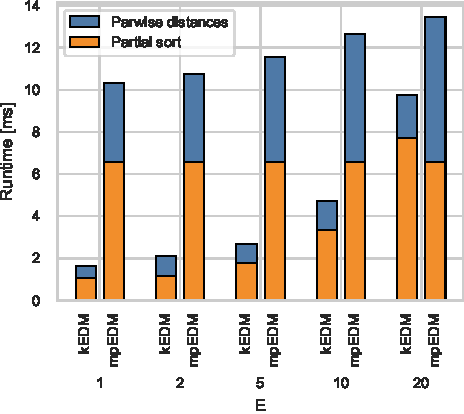
\includegraphics{figs/breakdown_v100}
    \caption{Breakdown of kNN runtime on V100}%
    \label{fig:architecture}
\end{figure}

\begin{figure}
    \centering
    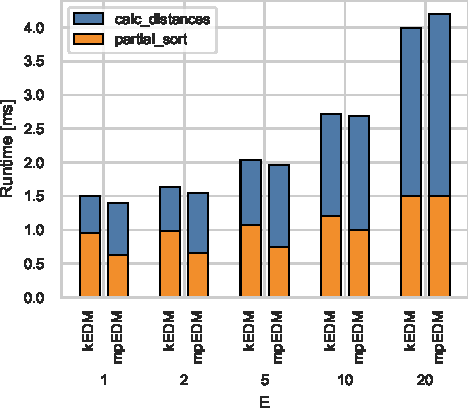
\includegraphics{figs/breakdown_epyc}
    \caption{Breakdown of kNN runtime on EPYC 7742}%
    \label{fig:architecture}
\end{figure}

\subsection{Efficiency}

Empirical Roofline Toolkit (ERT)\footnote{\url{https://bitbucket.org/berkeleylab/cs-roofline-toolkit/}}

\begin{figure}
    \centering
    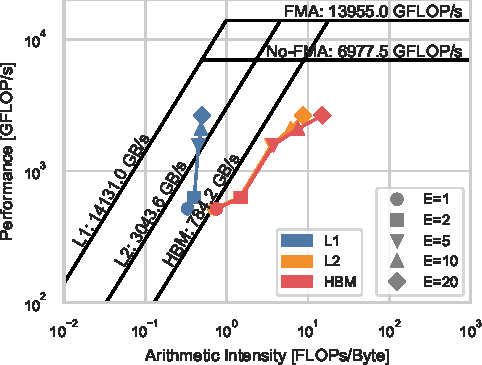
\includegraphics{figs/roofline_distances_v100}
    \caption{Roofline analysis of pairwise distance kernel on V100}%
    \label{fig:architecture}
\end{figure}

\begin{figure}
    \centering
    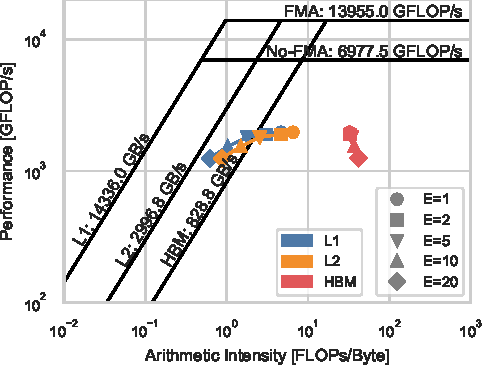
\includegraphics{figs/roofline_lookup_v100}
    \caption{Roofline analysis of lookup kernel on V100}%
    \label{fig:architecture}
\end{figure}

\begin{figure}
    \centering
    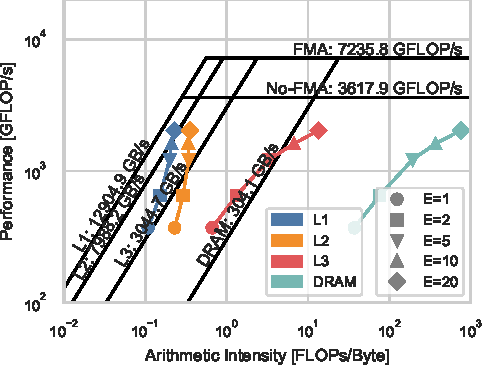
\includegraphics{figs/roofline_distances_epyc}
    \caption{Roofline analysis of pairwise distance kernel on EPYC 7742}%
    \label{fig:architecture}
\end{figure}

\begin{figure}
    \centering
    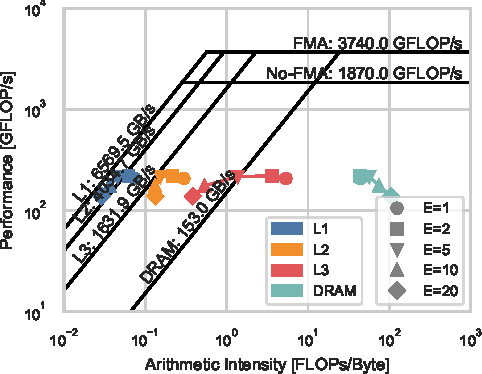
\includegraphics{figs/roofline_lookup_epyc}
    \caption{Roofline analysis of lookup kernel on EPYC 7742}%
    \label{fig:architecture}
\end{figure}

\section{Conclusion \& Future Work}

\section*{Acknowledgements}
This work was supported by JSPS KAKENHI Grant Number JP20K19808.

\bibliographystyle{IEEEtran}
\bibliography{references}

\end{document}
